 \providecommand{\main}{..}
\documentclass[\main/main.tex]{subfiles}
\begin{document}
\chapter{Problema del massimo flusso}
\section{Algoritmo di Ford e Fulkerson}
Si tratta di un algoritmo per calcolare il \textbf{massimo flusso} su un grafo da un nodo sorgente $s$ ad un nodo destinazione $t$.

\begin{definition}[Cammino incrementante]
  Un \textbf{cammino incrementante} è un cammino che ha archi con direzione positiva non pieni o archi con direzione negativa non vuoti.
\end{definition}

L'algoritmo procede nel modo seguente:

\begin{enumerate}
  \item Si identifica un cammino aumentante.
  \item Si identifica la capacità di strozzatura, cioè quella che su questo specifico cammino limita la capacità massima.
  \item Si aumenta la capacità occupata di ogni arco ed il flusso totale della differenza, ciò significa che in un cammino inverso (con freccia nella direzione inversa del flusso) il valore di flusso cala.
  \item Si ripete sino a che non è più possibile identificare un cammino aumentante.
\end{enumerate}

\section{Taglio di capacità minima}
Si tratta dell'insieme di archi che va da un sottoinsieme di nodi $\mathcal{P}_1$ ad un secondo sottoinsieme $\mathcal{P}_2$, con il totale dei nodi $\mathcal{P} = \mathcal{P}_1 \cup \mathcal{P}_2$ e $\mathcal{P}_1 \cap \mathcal{P}_2 = \emptyset$, cioè nessuno dei nodi in $\mathcal{P}_1$ si trova anche in $\mathcal{P}_2$ costruito in modo tale che esso limiti la capacità massima di flusso (insieme degli archi di strozzatura) che può andare dal nodo $s$ a $t$.

Un bel sito web che risolve questo problema è \url{https://bl.ocks.org/estk/9629395}.

\section{Flusso massimo a costo minimo}
Si tratta di riportare ogni arco $ij$ del digrafo tra un nodo $i$ e $j$, definito come $(u_{ij},c_{ij},x_{ij})$, dove $u_{ij}$ è la massima capacità di flusso dell'arco, $c_{ij}$ il costo per unità dell'arco e $x_{ij}$ la quantità di flusso che effettivamente scorre sull'arco, ad una forma a due archi come segue:

\begin{figure}
  \begin{subfigure}{0.49\textwidth}
    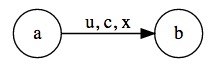
\includegraphics[width=0.8\textwidth]{g1}
    \caption{Arco con massima capacità $u$, costo $c$ e flusso inviato $x$.}
  \end{subfigure}
  \begin{subfigure}{0.49\textwidth}
    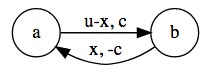
\includegraphics[width=0.8\textwidth]{g2}
    \caption{Archi con flusso inviato e costo}
  \end{subfigure}
  \caption{Flusso massimo a costo minimo}
\end{figure}

Una volta sostituiti tutti gli archi (nei temi d'esame è possibile compilare degli archi forniti) è necessario identificare circuiti in cui la somma dei costi è negativa.

Se questi esistono, il costo non è minimo ed è possibile ridurlo re-instradando il flusso del circuito identificato.

\section{Algoritmo di Prim}
Nell'algoritmo di Prim si procede con un metodo greedy: dato un set di nodi iniziali (spesso solo uno), a ogni step si sceglie il nodo con distanza minima connesso a uno dei nodi del set, lo si aggiunge al set e si ripete sino ad ottenere un albero ricoprente.

\end{document}